\subsubsection*{High inertial effects }
We now turn our attention to the high inertial regime ($Ga =100$).
In this situation it is expected that the presence of significant particles wake modify the interactions between particles \citep{yin2006}. 
\begin{figure}[h!]
    \centering
    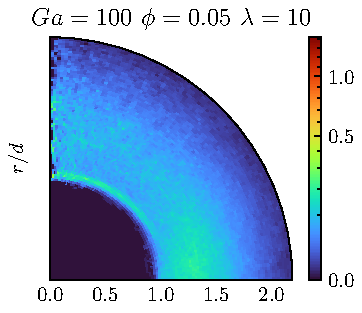
\includegraphics[height=0.21\textwidth]{image/HOMOGENEOUS_NEW/Dist/Pnst_l_10_Ga_100_PHI_0_05.pdf}
    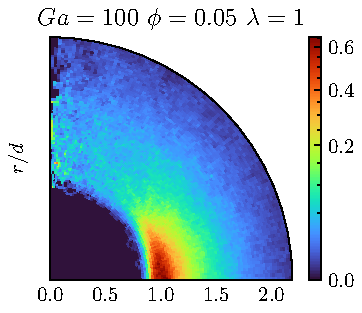
\includegraphics[height=0.21\textwidth]{image/HOMOGENEOUS_NEW/Dist/Pnst_l_1_Ga_100_PHI_0_05.pdf}
    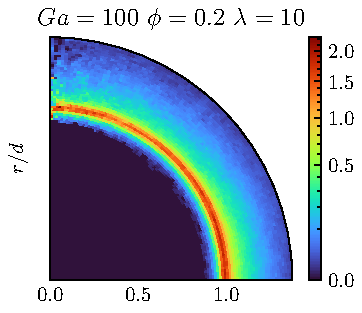
\includegraphics[height=0.21\textwidth]{image/HOMOGENEOUS_NEW/Dist/Pnst_l_10_Ga_100_PHI_0_2.pdf}
    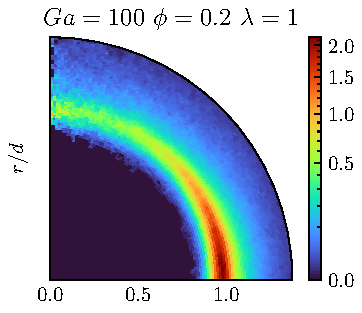
\includegraphics[height=0.21\textwidth]{image/HOMOGENEOUS_NEW/Dist/Pnst_l_1_Ga_100_PHI_0_2.pdf}
    \caption{Histogram of the normalized function $P_\text{r}^n$ at high inertial effects $Ga = 100$.
    The color map represents the values of the nearest pair distribution function. %of $P_\text{r}^n$.
    The origin corresponds to the position of the test particle.
    The dimensionless radial and azimuthal coordinates, $|\textbf{r}|/d$ and $\theta$, correspond to the nearest neighbor position.
    The vertical direction corresponds to the flow direction, which is also the axis of symmetry for $P_\text{r}^n$.
    (left) Low volume fraction cases $\phi=0.05$ for $\lambda = 1,10$.
    (right) High volume fraction cases $\phi=0.2$ for $\lambda = 1,10$.}
    \label{fig:Pnst_high_Ga}
\end{figure}
%If we compare \ref{fig:Pnst_high_Ga} (right) with their counterparts from \ref{fig:Pnst_low_Ga} (right) we observe that $P^n_\text{r}$ becomes even larger at contact of the particles for $Ga=100$.
%Again, this could witness of the presence of clustering of particles. 
%In general, all $P_\text{r}^n$ from \ref{fig:Pnst_high_Ga} exhibit some differences compared to the cases \ref{fig:Pnst_low_Ga}. 
%In the high inertial cases (\ref{fig:Pnst_high_Ga}), we can notice that $P_\text{r}^n$ is larger on the sides of the test particle for the iso-viscous emulsions ($\lambda = 1$).
Particularly striking, is the presence of anisotropy in \ref{fig:Pnst_high_Ga} for $\lambda=1$, compared to \ref{fig:Pnst_low_Ga}. In the former a higher concentration of particles is identified at $\theta \approx 0$, as seen in \ref{fig:Pnst_high_Ga}. In practice, a higher concentration of $P_r^n$ around $\theta \approx 0$ indicates the presence of horizontal rafts of particles. 
In this case, the microstructure is non-homogeneous and anisotropic, this situation is illustrated in \ref{fig:scheme_clusters} (\textit{Case 3}).  
Consequently, as the \textit{Galileo} number ($Ga$) increases and for low values of the viscosity ratio ($\lambda$), the probability of having neighbors on the horizontal plane of the test particle increases. 
This leads to an increase in the anisotropy of the microstructure which is more pronounced for low volume fraction. The high viscosity drops display an isotropic distribution of nearest particles around the test particle. This observation suggests the presence of isotropic clustering of particles.



%In comparison the high viscosity drops show an isotropic discitrbution of nearest particle around the test particle. This could witness of the presence of isotropic clustering of particles.

%We do not observe a significant effect of the volume fraction on the anisotropy of the distribution.
%However, at this stage it remains unclear if increasing $\phi$ have a positive or negative impact on the anisotropy of the distribution. 

To illustrate the impact of $\lambda$ on the microstructure, \ref{fig:images} displays snapshots of two DNS at $\phi = 0.05$ and $Ga = 100$. 
As predicted by $P_\text{r}^n$, we observe layers and particles in close contact for $\lambda = 1$, contrasting with the seemingly more evenly dispersed microstructure for $\lambda = 10$.
\begin{figure}[h!]
   \centering
   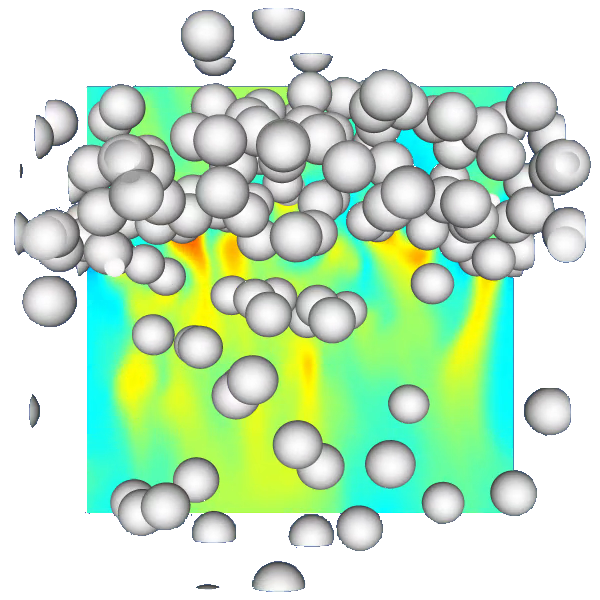
\includegraphics[width=0.4\textwidth]{image/HOMOGENEOUS_NEW/P_PHI_5_l_10_Ga_100.png}
   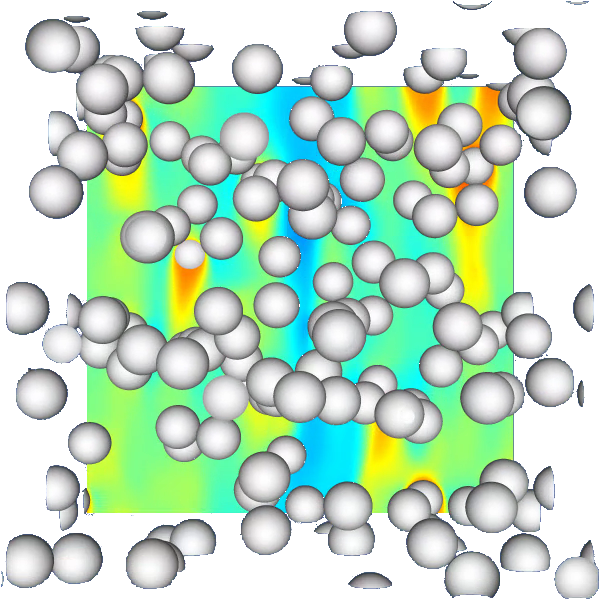
\includegraphics[width=0.4\textwidth]{image/HOMOGENEOUS_NEW/P_PHI_5_l_1_Ga_100.png}
   \caption{Snapshot of a simulation at $t^* = 150$ for $\phi=0.05$ and $Ga=100$.
   Color map : values of the vertical component of the velocity, field on the vertical plane defined by the equation $z=0$. 
   (left)  $\lambda = 1$.
   (right)  $\lambda = 10$.
   }
   \label{fig:images}
\end{figure}
In fact, for $\lambda = 10$, in \ref{fig:images} (right), we can still observe horizontal rafts of droplets or droplets rising side-by-side, but this effect is clearly not as pronounced as for $\lambda = 1$. 
Clearly, drops with high viscosity ratio maintain a significant distance between other drops, which prevent the creation of structures such as droplets layers.
This might be because of a higher vorticity around the viscous droplets.   
As discussed in \citet{zhang2021three}, rising pairs of spherical bubbles may reach a stable side-by-side configuration, which tends to generate horizontal clusters.
They range of dimensionless parameters is consistent with the ones presented in this study, making this hypothesis valuable. 
In \citet{legendre2003hydrodynamic} they study the interaction of a bubble pair rising side-by-side. 
They stipulate that for two bubbles at moderate \textit{Reynolds} number $50-100$, the interaction forces are found to be repulsive, while it is attractive or null for higher \textit{Reynolds} number. 
In our case it is reasonable to think that such pair attraction / repulsion mechanisms might drive the clustering mechanism.

%On another note, we can observe on \ref{fig:images} (left) that the distance between the layers is roughly equal to the length of the numerical domain. 
%Indeed, only one layer of droplets is present in the domain. 
%Therefore, the current microstructure is constrained by the size of the numerical domain, it is probably not representative of the real microstructure that we would obtain in an infinite non-periodic domain. 
%Additionally, one might argue that the layers appear due to collective effects drove by the size of the box.
%Indeed, it is exactly what we observe for small number of bubbles ($N_b = 4$) rising in a periodic domain, see \citet{loisy2017}. 
%However, we might expect that horizontal layers such as the one observed in \ref{fig:images} (left) still remain for lager boxes since the number of droplets is consequent.
%In our case, the presence of horizontal raft might be the consequence of pairwise interactions mechanism, as discussed above. 
%Therefore, it is likely that that layers still appear regardless of the size of the box.
%Nevertheless, the distance between these layers is still constrained by the size of the numerical domain, despite the consequent number of droplets used here. 
%In all rigor, DNS in a larger domain with more particles would be required to evaluate the microstructure dependence on the domain size. 
%Nevertheless, due to evident numerical constrains it has not been performed in this study.  
From the present analysis of $P_\text{r}^n$ and the actual microstructure presented in \ref{fig:images} we can infer that the \textit{nearest particle statistics} is able to predict features in the microstructure such as layers and clustering effects. 
Which is notable given that, to the author knowledge, no previous studies ever shown such visual proof in the context of the nearest neighboring statistics. 


\subsubsection*{Nearest radial distribution function }

Although, \ref{fig:Pnst_high_Ga} and \ref{fig:Pnst_low_Ga} give a good qualitative representation of the particle pair azimuthal distribution, they fall short in delivering a quantitative depiction of the radial distribution. %they do not provide a quantative representation of the radial distribution. %in details the differences in the radial distribution.
For a random isotropic distribution of hard spheres it is possible to derive a theoretical prediction for $P_\text{r}^n(r)$ obtained in the vanishing volume fraction limit. 
Indeed, it is shown in \citet{zhang2021ensemble} that for a dilute random arrangement of particle $P_\text{r}^n(r)$, reads as, 
\begin{equation}
    P_\text{r}^\text{th}(r) = \exp[{-4 \pi n_p (r^3 - d^3)/3}].
    \label{eq:Pnst_dilute}
\end{equation}
It must be understood that this formula is accurate only at $\mathcal{O}(\phi)$ therefore in most of our cases it is not expected to be representative.
Another theoretical distribution have been derived by \citet{torquato1990nearest} for arbitrary volume fraction $\phi$. 
In our notation it yields, 
\begin{equation}
    P_\text{r}^\text{torq}(r) = 
        \frac{6 \phi}{n_p \pi r^2 d}
        (er^2+f r+g)
    \exp\left[-\phi(8e(r^3-1)+12 f(r^2-1)+24g(r-1))\right]
\end{equation}
with, 
\begin{align*}
    && e= \frac{1+\phi}{(1-\phi)^3},
    && f= \frac{-\phi (3+\phi)}{2(1-\phi)^3},
    && g= \frac{\phi^2}{2(1-\phi)^3}.
\end{align*}
In both cases, the hard sphere model differ from the droplets pair distribution.
Indeed, in the latter case $P_\text{r}^\text{th} = 0$ for $r<d$ while in our case particles might deform at contact, meaning that $P_\text{r}^\text{th}$ is finite for certain $r<d$. 
However, it remains valuable to use these theoretical probability density function for comparative purposes. 

\begin{figure}[h!]
    \centering
    % 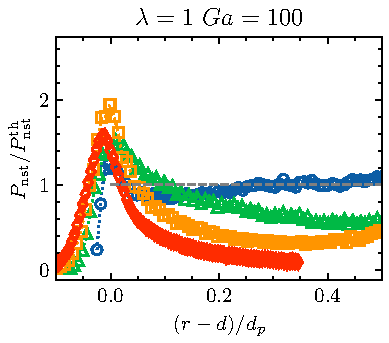
\includegraphics[height=0.3\textwidth]{image/HOMOGENEOUS_NEW/Dist/Pr_l_1_Ga_100.pdf}
    % 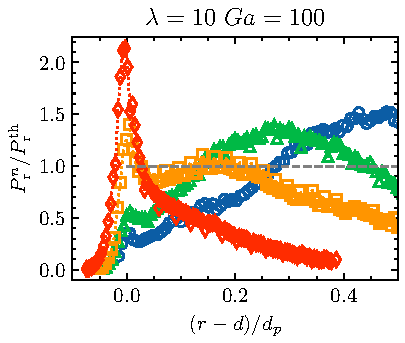
\includegraphics[height=0.3\textwidth]{image/HOMOGENEOUS_NEW/Dist/Pr_l_10_Ga_100.pdf}
    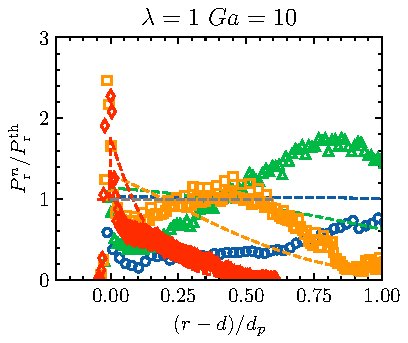
\includegraphics[height=0.3\textwidth]{image/HOMOGENEOUS_NEW/Dist/Pr_l_1_Ga_10.pdf}
    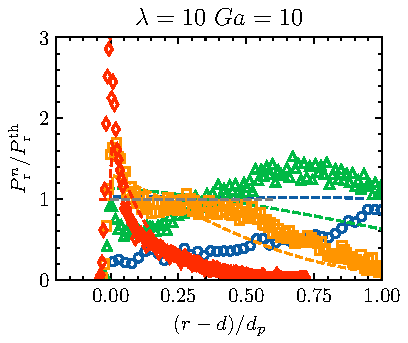
\includegraphics[height=0.3\textwidth]{image/HOMOGENEOUS_NEW/Dist/Pr_l_10_Ga_10.pdf}
    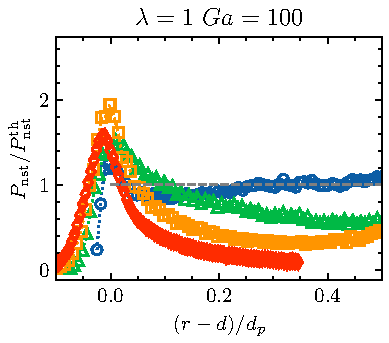
\includegraphics[height=0.3\textwidth]{image/HOMOGENEOUS_NEW/Dist/Pr_l_1_Ga_100.pdf}
    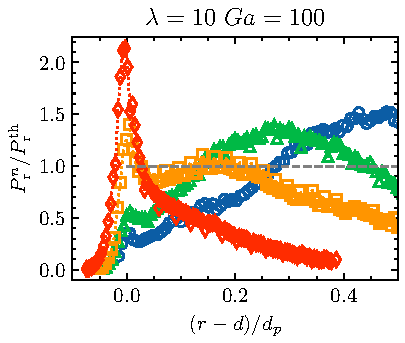
\includegraphics[height=0.3\textwidth]{image/HOMOGENEOUS_NEW/Dist/Pr_l_10_Ga_100.pdf}
    \caption{Radial probability density function $P_\text{r}^n(r)$ (symbols) and $P_r^\text{th}$ (dashed lines) divided by the theoretical distribution $P_\text{r}^{th}$ \ref{eq:Pnst_dilute}, in terms of the dimensionless distance $(r-d)/d$, for  $Ga = 100$.
    (left)  $\lambda = 1$.
    (right) $\lambda = 10$.
    ($\pmb\bigcirc$) $\phi = 0.01$; ($\pmb\triangle$) $ \phi = 0.05$; ($\pmb\square$) $\phi = 0.1$ ($\pmb\lozenge$) $\phi = 0.2$.
    (dashed lines) Theoretical prediction : $P_\text{r}^n/P_\text{nst}^\text{th} = 1$. 
    For $r<d$ we arbitrarily set $P_\text{r}^\text{th} = 1$ so that the distribution can be visualized.
    }
    \label{fig:Pr}
\end{figure}

In \ref{fig:Pr}  we plotted the radial distribution $P_\text{r}^n(r)$. %averaged on all $\theta$.
We displayed two different viscosity ratios and multiples volume fraction in terms of the dimensionless distance $(r - d)/d$ where $d$ is the particle diameter. 
In the dilute regime ($\phi = 0.01$) and for $\lambda=1$, we observe on \ref{fig:Pr} (left) that the radial distribution follow the dilute random arrangement of particle predicted by the theory (\ref{eq:Pnst_dilute}). 
In contrast when $\lambda = 10$ with the same $\phi$, it becomes evident that fewer particles gather in close vicinity to the test particle. Consequently, on average, the droplets are positioned at greater distances from each other compared to the dilute random distribution. %for $\lambda = 10$ at same $\phi$, we notice that less particles are in close proximity to the particle of refrence. Hence in average the drops are located further apart from each other in comparison to the dilute random distribution. 
For most of $\phi$ except $\phi=0.2$, we observe that the nearest particle distribution is higher at the contact of the particle of reference ($(r-d)/d = 0$), for $\lambda = 1$ than $\lambda = 10$. 
%Although, we selected a small \textit{Bond} number ($Bo = 0.2$), 
It is clear from \ref{fig:Pr} that the particles deform at contact, as witnessed by the non-vanishing value of $P_\text{r}$ for $(r-d)/d<0$.
%This is not surprising considering that $We \approx 0.6$ in these cases. 
%Therefore, in opposition to what stated in \ref{sec:methodo}, smaller bond number might eventually impact the particles' distribution at these $Ga$. 
%Nevertheless, in \ref{ap:age}, we displayed the same radial distribution but at $Ga =10$, see \ref{fig:Pr_low}. 
%It is clear that in these cases the particles do not deform at contact, making our hypothesis valid in this regime.
%Lastly, For high volume fraction ($\phi=0.2$) the distribution indicate a higher peak at contact of the test particle $(r-d)/d_p \approx 0$. 

In brief, we observed that both, the radial and azimuthal distribution were affected by the inertial effect measured by the \textit{Galileo} number. 
The major effect coming with high inertia is the generation of strong anisotropy in the particle pair distribution, as well as a more important concentration of neighboring particles at $(r-d)/d_p < 0$. 
Furthermore, for increasing volume fraction, the density at contact of the test particle is higher. 
Regarding the viscosity ratio, it has a strong impact on the microstructure, but only at high $Ga$, whereas at low $Ga$ the change in viscosity ratio has no notable impact on $P_\text{r}$, as seen in \ref{fig:Pnst_low_Ga} and \ref{fig:Pr_low}. 

\subsubsection*{Macroscopic modeling of the microstructure}
Up to now, we have presented visualizations of the microstructure with 2D or 1D distributions. 
However, for a more concise description, we would like to adopt a different approach. 
Following \citet{zhang2023evolution}, we opt to describe the microstructure using the second moment of $P_\text{nst}$ with respect to \textbf{r}, it reads,
\begin{equation}
    \textbf{R}(\textbf{x},t) =\frac{1}{n_p(\textbf{x},t)} 
    \int_0^\infty 
    \int_{\mathbb{R}^3} \textbf{rr} P_\text{nst}(\textbf{x},\textbf{r},t,a) d\textbf{r} da.
    \label{eq:R}
\end{equation}
This second-rank tensor measures the spread of the nearest neighbor distribution in a given direction. 
It's worth noting that such a quantity is computable only because $\lim_{|\textbf{r}|\to \infty} P(\textbf{x},\textbf{r},t,a) = 0$, which enables the integral of \ref{eq:R} to converge. 
This wouldn't be the case for classic pair distributions, which is the primary reason why we use the \textit{nearest particle statistics} framework. 

Since our objective is to measure the anisotropy of the microstructure, we are particularly interested in the deviatoric part of this tensor, namely,
\begin{equation*}
    \textbf{A}(\textbf{x},t) = \textbf{R}(\textbf{x},t) - \frac{1}{3} [\textbf{R}(\textbf{x},t) : \textbf{I}] \textbf{I}.
\end{equation*}
The tensor $\textbf{R}(\textbf{x},t)$ permits us to measure the mean square distance between a particle and its nearest neighbor, in average and in the three dimension of space. 
Therefore, $\textbf{A}(\textbf{x},t)$ represents likelihood of having a particle in a given direction compared to the mean radial square distance. 
Thus, for an isotropic suspension $A_{xx} = A_{xx} = 0$. 
In a scenario such as the one in \ref{fig:images} (left), it's evident that $A_{yy} < 0 < A_{xx} \approx A_{zz}$, as a particle is more likely to have its nearest neighbor situated on the sides, rather than on the verticals.
For a better interpretation of the following results it is of interest to compute the distance $r_m$, which is the mean distance to the nearest neighboring particle in a random distribution of hard sphere. 
By direct integration of \ref{eq:Pnst_dilute} we find, 
\begin{equation*}
    r_m^2 /d^2
    = \frac{1}{d^2n_p} 
    \int_{\mathbb{R}^3} r^2 P_\text{r}^\text{th}(r) d\textbf{r} 
    = {{4^{{{2}\over{3}}}\,\Gamma\left({{5}\over{3}} , 8\,\phi\right)
    \,e^{8\,\phi}}\over{2^{{{10}\over{3}}}\,\phi^{{{2}\over{3}}}}}
\end{equation*}
where $\Gamma(z,a) = \int_a^\infty t^{z-1} e^{-t} dt$ is the upper incomplete gamma function. 

\begin{figure}[h!]
    \centering
    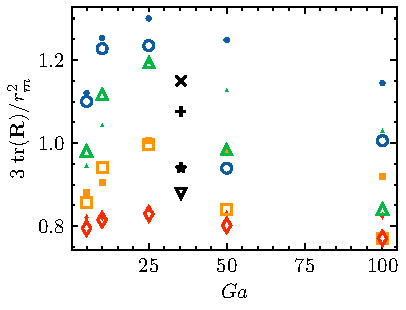
\includegraphics[height=0.3\textwidth]{image/HOMOGENEOUS_NEW/PA/trR.pdf}
    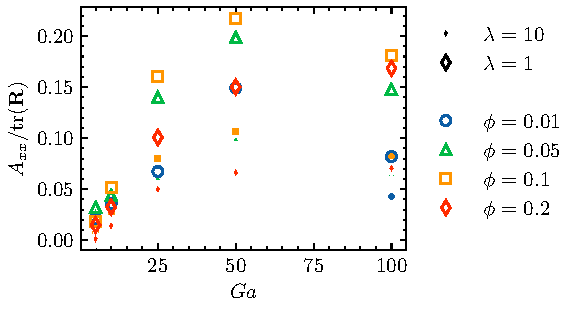
\includegraphics[height=0.3\textwidth]{image/HOMOGENEOUS_NEW/PA/Axx.pdf}
    \caption{
        (left) Trace of the second moment of the probability density function $P_\text{r}(\textbf{r})$ divided by the square diameter of the particles $d^2$. 
        (right) horizontal components of the anisotropy tensor divided by the trace of the second moment of the probability density function.
    ($\pmb\bigcirc$) $\phi = 0.01$; ($\pmb\triangle$) $ \phi = 0.05$; ($\pmb\square$) $\phi = 0.1$ ($\pmb\lozenge$) $\phi = 0.2$.
    The hollow symbols correspond to $\lambda = 1$, the filled symbols to $\lambda = 10$.
    For $r<d$ we arbitrarily set $P_\text{r}^\text{th} = 1$ so that the distribution can be visualized.
    Black symbols represent the results of \citet{zhang2023evolution} for hard sphere suspension with $\phi = 0.016,0.056,0.134,0.262$  %$\phi = 0.0168,0.0565,0.1341,0.2622$ 
    corresponding to $\pmb\times,\pmb +, \pmb\star , \pmb\triangledown$, respectively.
    }
    \label{fig:A}
\end{figure}
\ref{fig:A} (left) displays the value of the dimensionless mean square distance : $\textbf{I}:\textbf{R}/r_m^2$, between nearest neighbors for all our numerical cases. 
To help comprehension, first notice that the simulation denoted by the symbol \textcolor{col1}{$\pmb\circ$} in \ref{fig:A} (left), corresponding to $\lambda = 1$, $Ga = 100$ and $\phi = 0.01$, has a value of $\textbf{I}:\textbf{R}/r_m^2 \approx 1$. Which is consistent with the quasi hard sphere distribution reported for this case in \ref{fig:Pr} (left). 
It is clear from the graph that the mean square distance is mainly dependent on the volume fraction. 
We observe that $\textbf{I}:\textbf{R}/r_m^2$  decrease for increasing $\phi$, which means that particles get in average closer to one another compared to a hard sphere random distribution. 
As noted by \citet{zhang2023evolution} this implies the apparition of clusters as the particles get packed. 
Regarding the dependence on the \textit{Galileo} number, it is non-monotonic. 
Indeed, $\textbf{I}:\textbf{R}/r_m^2$ increase until $Ga = 25$ and then decrease until $Ga = 100$.  
% At rather high $Ga$ one might notice that the mean square distance for $\lambda = 1$ (hollow symbols) is lower. 
For most of our DNS we observe that the distance to the nearest neighbor for iso-viscous emulsions is on average greater for $\lambda = 10$, which is consistent with the distributions displayed in \ref{fig:Pr} and the picture from \ref{fig:images}.  
On \ref{fig:A} (left) the symbols : $\pmb\star, \pmb\times,\pmb +, \pmb\triangledown$, represent the results of \citet{zhang2023evolution} for hard sphere sedimentation. 
As observed, the value of $\textbf{R}:\textbf{I}$ is on average closer to the mean $r_m^2$ than our simulations, but it maintains the same trend, i.e., clusters appear as the volume fraction increases.

 
Regarding the anisotropy measure we can see on \ref{fig:A} (right) that we have $A_{xx} \ge 0$ for nearly all our cases, meaning that globally, the emulsion is either isotropic ($A_{xx} = 0$), or with particles that are in average more aligned horizontally ($A_{xx} >0$). 
Then, we can see that $A_{xx}$ increase until $Ga = 50$ where we reach a maximum, and then decrease until $Ga =100$  but still remains consequent. 
Consistently with the cases from \ref{fig:images}, the value of $A_{xx}$ is greater for $\lambda = 1$ lower for  $\lambda = 10$.
Although, it is not quite obvious we observe a non-monotonic trend with the volume fraction, $A_{xx}$ first increases up to a maximum value for $\phi =0.1$ (represented by \textcolor{col3}{$\pmb\square$} on \ref{fig:A} (right)) and then decreases for $\phi=0.2$ (represented by the \textcolor{col4}{$\pmb\lozenge$} symbols). 
This implies that at a certain volume fraction, around $\phi \approx 0.1$, higher $\phi$ makes the microstructure more isotropic, while at low volume fraction ($\phi < 0.1$) increasing $\phi$ favors the side-by-side configuration.
This phenomenon of isotropization at high $\phi$ has been reported in other studies such as in \citet{seyed2021sedimentation} for sedimentation of solid particles. 
However, at high \textit{Galileo} number it seems that this effect is less pronounced. 


We conclude that the microstructure can be classified into three classes :
(1) The homogeneous microstructure. 
(2) The non-homogeneous but isotropic microstructure. 
(3) The non-homogeneous and non-isotropic microstructure. 
Each of these types are characterized with specific values of $\textbf{R}(\textbf{x},t)$, they are reported in \ref{tab:microstructure}. 
Additionally, to better visualize the dependence of $\textbf{R}(\textbf{x},t)$ on $\phi$ and $Ga$, we display the values of $A_{xx}/tr(\textbf{R})$ and $\textbf{R}:\textbf{I}/r_m^2$ in phase diagrams on \ref{fig:phase}.
In short, we observe that the mean square particle distance compared to a random case is decreasing with the volume fraction, and is globally higher for viscous particles ($\lambda = 10$).
Meanwhile, the likelihood of finding the nearest neighboring particle on the horizontal is greater for $\lambda=1$ than $\lambda = 10$, and it is globally increasing with higher $Ga$ and non-monotonic with $\phi$. 
It is seen that at $Ga \approx 50$ and $\phi \approx 0.1$ we reach the configuration with the maximum anisotropy for both $\lambda$. 
\begin{table}[h!]
    \caption{Microstructure classification}
    \label{tab:microstructure}
    \centering
    \begin{tabular}{|lccccc|} \hline
        Types & Homogeneous & Isotropic & \ref{fig:scheme_clusters} & $\textbf{R}:\textbf{I}/r_m^2$ & $A_{xx}/tr(\textbf{R})$ \\
        Homogeneous & Yes & Yes &(\textit{Case 1}) & $\geq 1$ & $\ll 1$ \\
        Clustering &  No & Yes  &(\textit{Case 2}) & $ < 1$ & $\ll 1$ \\
        Layering &    No & No  &(\textit{Case 3}) & $ - $ & $< 1$\\ \hline
    \end{tabular}
\end{table}
\begin{figure}[h!]
    \centering
    \begin{tikzpicture}[scale=0.8]
        \node (img) at (0,0) {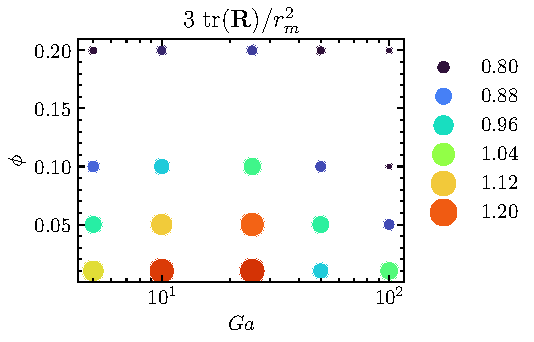
\includegraphics[height=5.5cm]{image/HOMOGENEOUS_NEW/PA/phase_Rtr_l_1.pdf}};
        % \draw[dashed] (10cm,-1.6) ellipse (3 and 2);
        \node (txt) at (-2,1) {Clustering};
        \node (txt) at (-1,-1.6) {Evenly dispersed};
        \draw[dashed] ($(-1,-1.6) + (-10:3 and 2)$(P) arc
        (-10:155:3 and 2);
        \node (img) at (10.5,0) {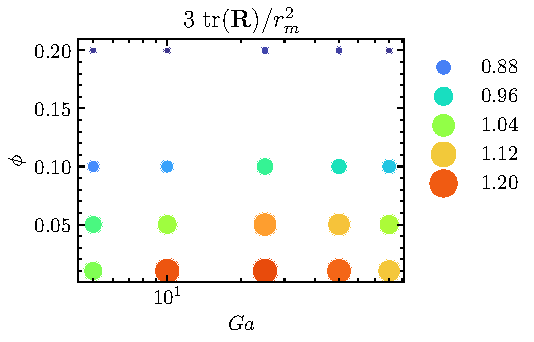
\includegraphics[height=5.5cm]{image/HOMOGENEOUS_NEW/PA/phase_Rtr_l_10.pdf}};
        % \draw[dashed] (10cm,-1.6) ellipse (3 and 2);
        \node (txt) at (8.5,1) {Clustering};
        \node (txt) at (10,-1.6) {Evenly dispersed};
        \draw[dashed] ($(10,-2) + (-10:3 and 2)$(P) arc
        (-10:180:3 and 2);
    \end{tikzpicture}
    \begin{tikzpicture}[scale=0.8]
        \node (img) at (0,0) {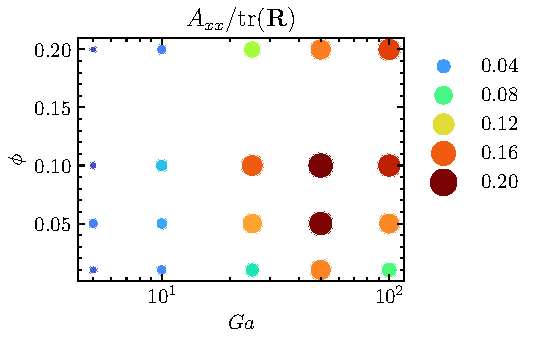
\includegraphics[height=5.5cm]{image/HOMOGENEOUS_NEW/PA/phase_axx_l_1.pdf}};
        \draw[dashed] (1.2,0.3) ellipse (1.5 and 2.5);
        \node (txt) at (1.2,1) {Anisotropic};
        \node (txt) at (-2,1) {Isotropic};

        \node (img) at (10.5,0) {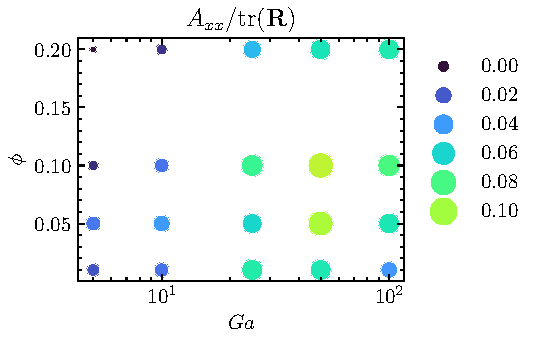
\includegraphics[height=5.5cm]{image/HOMOGENEOUS_NEW/PA/phase_axx_l_10.pdf}};
        % \draw[dashed] (11.7,-0.5) ellipse (0.75 and 1.75);
        % \node (txt) at (11.7,1) {Anisotropic};
        \node (txt) at (8,1) {Isotropic};
    \end{tikzpicture}
    \caption{
        (top) Phase diagram of the dimensionless mean square distance to the nearest neighbor, $(\textbf{R}:\textbf{I})/r_m^2$.
        (bottom) Phase diagram of the dimensionless horizontal components of the anisotropy tensor, $A_{xx}/\text{tr}(\textbf{R})$.  
        (left) Iso-viscous emulsion $\lambda = 1$.
        (right) Viscous droplets $\lambda = 10$ }
    \label{fig:phase}
\end{figure}

Although, previous studies mainly focused on bubbles or solid particles, it is reasonable to compare the $\lambda = 1$ and $\lambda = 10$ simulations, to the former and the latter cases, respectively. 
In \citet{bunner2002dynamics} they performed tri-periodic simulation of buoyant bubbles at $Re \approx 10-30$ for various $\phi$.
They reported a preference for the bubbles to be aligned in pair. 
Which is consistent with what we observe in \ref{fig:phase} ($\lambda = 1$) since the anisotropy tensor : $A_{xx} \approx 0.15$, for $Ga = 25$ (which correspond roughly to $Re = 25$). 
% Additionally, it is seen that these layers structures are lost at lower volume fraction ($\phi = 0.01$). 
Furthermore, in \citet{zhang2021direct} they carried out DNS of buoyant bubbly flows in tri-periodic domains.
Their \textit{Reynolds} numbers range form $Re=22.5\to 18$ for various volume fraction : $\phi = 0.05\to 0.2$ and a fixed \textit{Galileo} number of $Ga = 29$. 
They observe anisotropic clusters for $\phi >0.1$ as well, and they report that at lower volume fraction these structures are not present. 
It is consistent with the results reported in \ref{fig:phase} (left) where we can see that the value of $A_{xx}$ clearly decreases for lower $\phi$. 

For solid particles at $Ga = 144$, it is observed in \citet{shajahan2023inertial} that in the dilute regime, ($\phi \approx 0.02$), verticals raft of particles are formed. 
In our case we could not observe such a phenomenon, meaning that it might arise at even higher viscosity ratio or \textit{Galileo} number. 
The latter effect is explained by the presence of a more developed wake for dilute solid particles which trap neighboring particles within the wake without repulsing it on the sides. 
In our case we observe more particles in the verticals directions for $\lambda = 10$ than $\lambda =1$ at $Ga =100$, since $A_{xx}$ is smaller in the former cases.
Although it is not quite obvious it might be the consequence of the same effects, i.e., the wake of the viscous drop might induce less side-by-side configuration and more vertical nearly stable configuration. 
DNS at higher $Ga$ and $\lambda$ would be necessary to confirm or not the presence of the wake trapping effect.  
In the moderately dense regime,  $0.02 < \phi \le 0.1$  \citet{shajahan2023inertial} identified more configuration of particles situated side-by-side. 
As mentioned above even if it is less pronounce than for $\lambda = 1$ we indeed observe that $A_{xx}$ is higher in these cases, see \ref{fig:phase} (right). 
Additionally, \citet{almeras2021statistics} carried experiments of liquid-solid fluidized bed with spherical particles. 
Their Reynolds numbers range between $150\leq Re \leq 360$ depending on the volume fraction $0.14 \leq \phi \leq 0.42$.
It is observed that particles are most concentrated on the horizontal plane of the test particle when $\phi = 0.14$.
If the $\lambda = 10$ cases follow the same trend, it is reasonable to expect that the probability of horizontal configurations, already predominant at $Ga =100$, will continue to increase for higher \textit{Galileo} at $\phi  \approx 0.1$. 


We would like to end this comparison with the literature with the study of \citet{yin2008lattice} which compares the microstructure of suspensions of rising bubbles with suspensions of sedimenting solid particles.
They studied two \textit{Reynolds} numbers and two volume fractions : $Re = 5,20$ and  $\phi = 0.05, 0.2$, respectively.
It is found that : 
\enquote{    
     microstructure in bubble
    suspensions is more anisotropic and inhomogeneous than
    solid particle suspensions of the same volume fraction and
    \textit{Reynolds} number.    
}. 
Although we compare emulsions with varying droplets' viscosity rather than bubbles and solid particles' suspension, our conclusion regarding the anisotropy of the flow is consistent with their study.
Additionally, it is also observed in \citet{yin2008lattice} that the microstructure shape has a clear impact on the mean rising velocity of the dispersed phase.
Indeed, they observed that a power-law function of $(1-\phi)$ fit perfectly the rising velocity of random and isotropic suspensions, while it is not the case when the microstructure exhibit anisotropic structures. 
Therefore, as stated in introduction, the knowledge of the microstructure shape (reported in \ref{fig:phase}), is of utmost importance in the objective of building realistic averaged models. 

Ultimately, \ref{fig:A} and \ref{fig:phase} constitutes a significant result of this work as it quantifies the microstructure geometry using only the second rank tensor $\textbf{R}(\textbf{x},t)$.
Upon a good estimation of the values of $\textbf{I}:\textbf{R}$ and $A_{xx}$ one is able to predict the presence of side-by-side arrangement and clustering effects. 
For future perspectives, based on the value of $\textbf{R}(\textbf{x},t)$, an approximation of the distribution $P_\text{r}(\textbf{x},\textbf{r},t)$ could be reconstructed by assuming a certain functional form with 2 degrees of freedom.
Each degree of freedom would correspond to the scalars, $\textbf{R}:\textbf{I}$ and $A_{xx}$.
This approximated distribution could then be used to take in account of the various microstructure in certain theoretical problems involving the theoretical pair distribution function (\citet{batchelor1972sedimentation}, \citet{hinch1977averaged}, and \citet{zhang2021ensemble}).

% In the following we try to explain the origin of the striking difference between $\lambda = 1$ and $\lambda = 10$ on the particle pair distribution.
% With this objective in mind, we present a meticulous analysis of the particle time of interaction as well as the particles relative averaged velocity fields. 
